\newtheorem{definition}{Definícia}[section]

\def\UrlBreaks{\do\/\do-}

\chapter{Úvod}

\chapter{Základné pojmy a definície}
Táto kapitola oboznamuje so základnými pojmami, ktoré vedú k pochopeniu obsahu tejto bakalárskej práce. Vzhľadom na to, že táto práca je úzko spätá s hudbou a hudobnou teóriou, obsahuje jej základy, ktoré sú prevzaté z \cite{MUSICTHEORY}, \cite{DunnettVar}. Základy formálných jazykov a ich definície sú prevzaté z \cite{MEDUNATHEORY}.

\section{Hudba}
Hudba je súčasťou umenia. Základným stavebným materiálom hudby je tón. Pomocou hudby sa skladateľ snaží vyjadriť nejakú myšlienku. Hudobnú myšlienku je možné zapísať notami pomocou notového zápisu. Cieľom tejto podkapitoly je objasnenie základných pojmov hudby, ako i ukážka hudobnej štruktúry téma a variácie.

\subsection{Tón}
Tón je definovaný, ako zvuk s určitou výškou a vzniká pravidelným chvením nejakého zdroja zvuku. Vzniknuté chvenie sa prenáša do sluchových orgánov zmenou hustoty vzduchu. Skladá sa z rôznych vlastností, ako sú výška, sila, farba a dĺžka. Najdôležitejšie vlastnosti sú výška tónu a jeho dĺžka, ktoré sú predmetom tejto práce.

Dĺžka tónu nie je narozdiel od ostatných vlastností fyzikálnou, ale je závislá od interpreta daného tónu. Čas znejúceho tonu je jeho dĺžka. Interpret jeho zásahom pri interpretácií vie určiť dĺžku tónu.

Výška tónu je definovaná ako počet kmitov za jednu sekundu. Spolu s výškou tónu sa zvyšuje počet kmitov za sekundu. Počet kmitov za jednu sekundu sa udáva v Hertzoch.

Tóny sú usporiadané do tónovej sústavy. Tónová sústava je množina tónov, ktoré sa v hudbe vyskytujú. Tvorí ju sedem základných tónov c, d, e, f, g, a, h. Tieto tony sú výškovo usporiadané od najnižšej po najvyššiu. Po tóne h vždy nasleduje tón c, ktorý má dvojnásobnú frekvenciu oproti tomu pôvodnému. Všetkých osem tónov tvorí oktávu. V tejto práci sú použité dve oktávy, a to sú jednočiarkovaná oktáva a dvojčiarkovaná oktáva.

Na obrázku \ref{fig:tonfrek} sú zobrazené tóny cez dve oktávy, ktoré sú pomenované. K príslušným tónom bola priradená ich frekvencia na základe \cite{strankaFrekvencii}. Môžeme na obrázku spozorovať, ako frekvencie tónov medzi oktávami súvisia. Jednočiarkovaná oktáva, ktorá sa začína tónom c a končí tónom c2 má polovičnú frekvenciu dvojčiarkovanej oktávy, ktorá sa začína tónom c2 a končí tónom c3. Jednotlivé tóny vieme posunúť o oktávu vyššie vďaka zdvojnásobeniu ich frekvencie.

\begin{figure}[H]
\centering
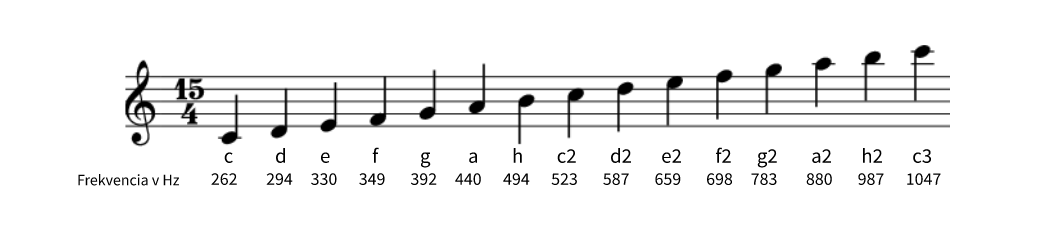
\includegraphics[scale=0.4]{obrazky-figures/Tonyafrekvencie.png}
\caption{Postupnosť tónovov cez dve oktávy s príslušnými frekvenciami.}
\label{fig:tonfrek}
\end{figure}

\subsection{Nota}
Nota je grafická značka, ktorá sa zapisuje do notovej osnovy. Pomocou noty vieme vyjadriť dĺžku tónu a jeho výšku. Ostatné vlastnosti tónu sa zapisujú inými značkami. Zápis nôt do notovej osnovy je potrebný pre reprezentáciu hudobnej myšlienky alebo jej interpretáciu. Noty majú rôzne značenie. Notu tvorí hlavička a nožička. V tejto práci sú použité tri základné značenia, ako sú celá nota, polová nota a štvrťová nota. Tieto notové značenia sú na obrázku \ref{fig:druhnot}.

\begin{figure}[H]
\centering
\includegraphics[scale=0.4]{obrazky-figures/Druhynôt.png}
\caption{Notové značenia.}
\label{fig:druhnot}
\end{figure}

\subsection{Takt}
Pod taktom v hudbe rozumieme základnú jednotku pravidelného striedania prízvučných a neprízvučných dôb. Určuje sa v notovom zápise, na začiatku skladby. Značený je dvomi číslami. Vrchné číslo určuje počet dôb v jednom takte. Spodné číslo označuje notu, ktorá trvá jednu dobu.

Na obrázku \ref{fig:dvojst} je dvojštvrťový takt, ktorý obsahuje dve dvojštvrťové noty c, d. Dvojka značí to, že v jednom takte sa môžu maximálne vyskytovať dve doby. Štvorka označuje trvanie štvrťovej noty, ktorá trvá jednu dobu. V tomto takte sa nemôže napríklad vyskytovať celá nota, ktorá trvá štyri doby a presahuje tak dĺžku jedného taktu.

\begin{figure}[H]
\centering
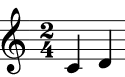
\includegraphics[scale=0.4]{obrazky-figures/dvojst.png}
\caption{Dvojštvrťový takt.}
\label{fig:dvojst}
\end{figure}


Obrázok \ref{fig:trojst} už obsahuje štvorštvrťový takt, v ktorom sa už môže vyskytovať celá nota, ktorá trvá štyri doby.

\begin{figure}[H]
\centering
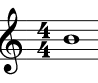
\includegraphics[scale=0.4]{obrazky-figures/cela.png}
\caption{Štvorštvrťový takt.}
\label{fig:trojst}
\end{figure}

\subsection{Notový zápis}
Notový zápis sa skladá z piatich čiar a štyroch medzier. Začína sa klúčom, ktorý slúži pre relatívne určenie výšky skladby. Existujú rôzne kľúče. V tejto práci sa vyskytuje jeden a tým je husľový kľúč. Husľovým kľúčom sa zapisujú tony stredné a vysoké. 

Po husľovom kľúči sa určí tónina. Tónina je množina tónov, ktorá je obsiahnutá v melódií. Každá tónina prislúcha nejakej stupnici. Stupnicu tvorí osem základných tónov, ktoré sú výškovo usporiadané. Stupnica sa začína tónom, ktorý prisluši názvu stupnici. C durová stupnica sa začína tónom c. V tejto práci sa pracuje čisto s notami z C durovej stupnice a výsledky práce sú v C durovej tónine.

Zapísaný kľúč a tóninu, v ktorej je melódia zapísaná nasleduje určenie taktového predpisu. Posledná časť notového zápisu je samotná melódia, ktorá je zapísaná notami.

V prípade, že k zápisu nôt do notovej osnovy nestačí počet čiar, potom sa pridávajú pomocné čiary. Príklad pomocnej čiary je pre notu c na obrázku \ref{fig:tonfrek}.

\subsection{Téma a variacie}
Téma a variácie sú bežné hudobné prostriedky, ktoré tvoria hudobnú štruktúru. Táto hudobná štruktúra je používaná vo veľkej miere v klasickej hudbe. Štruktúra je založená na téme, ktorá sa vyskytuje na začiatku hudobnej myšlienky. Potom, ako odznie téma prichádzajú na rad variácie. Variácia je obmena témy rôznymi spôsobmi. Tento proces je opakovaný niekoľkokrát. Ukončenie tohto procesu záleží na skladateľovi. Z vytvorenej variácie je stále možné vyzistiť originálnu tému, z ktorej bola variácia vytvorená. Proces tvorenia tejto hudobnej štruktúry je zobrazený na obrázku \ref{fig:Schemvar}.

\begin{figure}[H]
\centering
\includegraphics[scale=0.4]{obrazky-figures/SchémaVar.png}
\caption{Schéma aplikovania variácií.}
\label{fig:Schemvar}
\end{figure}

Tvorca hudobnej myšlienky môže k variovaniu témy využiť rôzne hudobné prostriedky. Medzi tieto prostriedky patrí zmena melódie. Melódia je hlavný výrazový prvok hudby, ktorý umožňuje vnímanie a pochopenie hudby. Melódia môže ovplyvniť aj náladu hudby. Variovanie melódie je možné vďaka pridávaniu tónov, odoberaním tónov alebo invertovanie melódie. Počas barokového obdobia sa stali populárne rôzne zdobenia tónov, ktoré môžu takisto variovať tému.

Ďalším spôsobom, ako vytvoriť variáciu témy je zmena rytmu melódie. Zmena rytmu melódie je aplikovaná na tému skladby. Vykonáva sa či už nad jednotlivými notami alebo nad celým taktom. Jednotlivým notám sa môže zvýšiť ich dĺžka alebo aj znížiť niekoľkonásobne. 

Medzi hudobné elementy, ktoré sa dajú zmeniť patrí aj harmónia a tonalita skladby. Cieľom tejto techniky je zmeniť tóninu hudby. V prípade, že skladba je písaná v tónine, ktorá je veselá sa zmení na smutnú. Toto sa dá aplikovať aj opačne a zmeniť smutnú tóninu na veselú. Veselé tóniny sa nazývajú durové a smutné sú molové. Samozrejme, že zmena tóniny je možná v rámci durových alebo molových tónin.

Vytvorenie ďalšej variácie je možné aj zmenou taktového predpisu. Zmenou taktového predpisu prepíšeme tému napríklad z dvoj štvrťového taktu na troj štvrťový takt. Spôsobí to zmenu usporiadania nôt v takte, vďaka tomu, že sa do jedného taktu zmestí počet nôt o jednu dobu kratší.

\subsection{Bežné druhy variácií}
Predmetom rôznych práci je práca s hudbou a analýza jej častí. Jednou z nich je práca \cite{variationRelevance}, ktorá sa zaoberá vyhľadávaním hudobnej kategórie v hudbe a relevantnosťou výsledku. Zistenie kategórie polyfónnej symbolickej hudby je založené na základe sémantického učenia konceptu hudby. Aby tento systém vzal do úvahy globálne, ale i lokálne vlastnosti hudobných objektov, prezentuje prístup k modelovaniu hudobného objektu na základe bázových segmentov. 

Modelovanie hudobného objektu sa skladá z viacerých části, prvá z nich je získanie potenciálne významných segmentov pre každý hudobný objekt. Ďalším krokom je pre každý významný segment hudobného objektu vybrať prvky lokálnej reprezentácie. Potom sú všetky významné segmenty vyberané na základe ich dôležitosti. Na základe dôležitosti sú vyberané dôležité objekty z tých objektov, ktoré boli označené ako potenciálne dôležité. Posledným krokom je pre každý hudobný objekt získať reprezentácie globálnej vlastnosti.

V hudbe motív, ktorý je výrazne sa opakujúci segment nôt sa používa na zloženie časti alebo celej témy. Opakovanie tohto motívu môže mať nejaké variácie, ktoré nemusia byť vždy presnou kópiou hudobného objektu. Tieto opakujúce sa vzory vo variáciách sa nazývajú motivické opakujúce sa vzory. Tieto motivicky sa opakujúce vzory môžu byť potenciálne dôležité segmenty pre charakterizovanie melódie hudobného objektu.  

Preto v tejto práci bolo použitých šesť bežných druhov motívových variácií podobne ako v \cite{variationRelevance}. Tieto motívové variácie sú: 

\begin{itemize}\itemsep0.05em
    \item Opakovanie je presne kopírovanie nôt do ďalšieho taktu ako je na obrázku \ref{fig:repetition}.
    \begin{figure}[H]
    \centering
    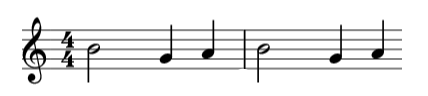
\includegraphics[scale=0.4]{obrazky-figures/rep.png}
    \caption{Obrázok opakovania taktu.}
    \label{fig:repetition}
    \end{figure}
    \item V transpozícii sa motív prenesie na ďalšiu úroveň kmitočtu. Napríklad nota h má kmitočet 494 Hz, takže na ďalšej úrovni bude mať dvojnásobný kmitočet 987 Hz. Príklad tohto posunu je na obrázku \ref{fig:transpozicia}.
    \begin{figure}[H]
    \centering
    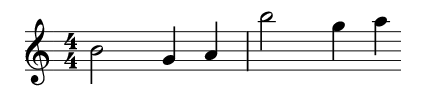
\includegraphics[scale=0.4]{obrazky-figures/trans.png}
    \caption{Obrázok transpozície taktu.}
    \label{fig:transpozicia}
    \end{figure}
    \item Postupnosť v tomto prípade znamená prenesenie motívu konštantne o jeden tón vyššie alebo o jeden tón nižšie. Na obrázku \ref{fig:Postupnost} je motív v druhom takte prenesený o jeden tón nižšie a v treťom takte je prenesený o jeden tón vyššie oproti prvému taktu.
    \begin{figure}[H]
    \centering
    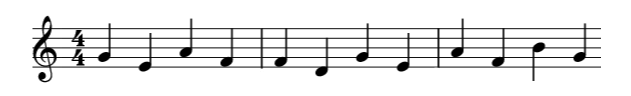
\includegraphics[scale=0.4]{obrazky-figures/Post.png}
    \caption{Obrázok postupného zvyšovania a znižovania pôvodného taktu.}
    \label{fig:Postupnost}
    \end{figure}
    \item V protipohybe sa zoberú intervaly z prvého taktu, ktorý je v tomto prípade motív. Potom v ďalšom takte sa tieto vzdialenosti tónov invertujú. V prvom takte na obrázku \ref{fig:Protipohyb} sú vzdialenosti medzi tónmi 2, -1, -2. V druhom takte sú vzdialenosti medzi tónmi -2, 1 a 2.
    \begin{figure}[H]
    \centering
    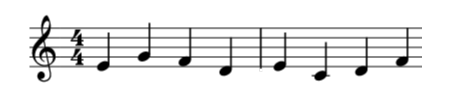
\includegraphics[scale=0.4]{obrazky-figures/Proti.png}
    \caption{Obrázok protipohybu pôvodného taktu.}
    \label{fig:Protipohyb}
    \end{figure}
    \item Retrogradácia v hudbe je zopakovanie nôt z pôvodného motívu v opačnom poradí. Napríklad, ako je motív v prvom takte na obrázku \ref{fig:Preklopenie} v poradí tónov d, g, e tak jeho variácia v druhom takte je e, g d.
    \begin{figure}[H]
    \centering
    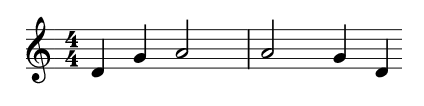
\includegraphics[scale=0.4]{obrazky-figures/Prek.png}
    \caption{Obrázok retrogradácie taktu.}
    \label{fig:Preklopenie}
    \end{figure}
    \item V prípade variovania témy predlžovaním alebo znižovaním dĺžky nôt je motív opakovaný. Variovanie motívu prebieha na obrázku \ref{fig:augmentacia} zdvojnásobením pôvodnej dĺžky noty. Keďže je stále potrebné dodržať rytmus taktu, tak sa museli posledné dve noty presunúť do extra taktu. Z taktového predpisu jeden takt môže obsahovať 4 doby. Po zdvojnásobení tejto dĺžky je potrebné rozložiť 8 dôb do dvoch taktov.
    
    Na obrázku \ref{fig:Diminution} je dvojnásobné zníženie dĺžky nôt. Keďže takt trvá 4 doby, potom jeho polovičné zníženie trvá 2 doby. Pre dodržanie tohto taktového predpisu je k dvom dobám pridaná pomlčka, ktorá trvá 2 doby.
    
    \begin{figure}[H]
    \centering
    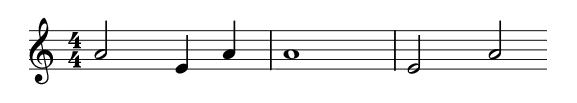
\includegraphics[scale=0.4]{obrazky-figures/Aug.png}
    \caption{Predĺženie dĺžky taktu.}
    \label{fig:augmentacia}
    \end{figure}
    \begin{figure}[H]
    \centering
    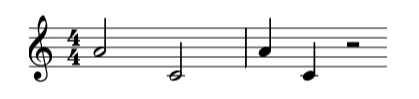
\includegraphics[scale=0.4]{obrazky-figures/Dimi.png}
    \caption{Skrátenie dĺžky taktu.}
    \label{fig:Diminution}
    \end{figure}
\end{itemize}

\section{Formálne jazyky}

\subsection{Množina}
Skupinu nejakých elementov, ktoré sú prevzaté z nejakého dopredu dohodnutého prostredia nazývame množinou $\Sigma$. Element a patrí množine M vtedy, ak sa v nej nachádza. Zapisujeme to ako $a \in \Sigma$. V prípade, že sa v množine nenachádza zapíšeme to ako $a \not \in  \Sigma$. Ak počet prvkov v množine vieme spočítať, potom o množine hovoríme, že je konečná. Ak prvky nespočítame, potom je množina nekonečná. Konečná množina, ktorá neobsahuje žiadne prvky je prázdna množina. Prázdnu množinu označujeme ako $\emptyset$.

Konečnú množinu $\Sigma$ môžeme špecifikovať vypísaním jej elementov. Obsah množiny zapíšeme ako $\Sigma = \{a_1, a_2, a_3, ..., a_n\}$, kde prvky $a_1, a_2, a_3, ..., a_n$ patria množine $\Sigma$.

V práci s množinami využívame rôzne operácie ako sú zjednotenie, prienik a rozdiel. Zjednotenie dvoch konečných množín $\Sigma$ a $\Omega$ definujeme ako $\Sigma \cup \Omega = \{a | a \in \Sigma \: alebo  \: a \in \Omega \}$, ich prienik $\Sigma \cap \Omega = \{a | a \in \Sigma \: z\acute{a}rove\check{n}  \: a \in \Omega \}$, a rozdiel $\Sigma \setminus \Omega = \{a | a \in \Sigma \: z\acute{a}rove\check{n}  \: a \not \in \Omega \}$.

\subsection{Abeceda}
Abecedou $\Sigma$ nazývame konečnú množinu, ktorá obsahuje prvky nazývané symbolmi.

\subsection{Reťazec}
Reťazcom nad abecedou $\Sigma$ nazývame konečnú postupnosť symbolov abecedy $\Sigma$. Reťazec, ktorý neobsahuje symboly sa nazýva prazdny reťazec a označujemeho ako $\varepsilon$

$\Sigma^*$ označuje množinu všetkých možných reťazcov nad abecedou $\Sigma$. $\Sigma^+$ označuje $\Sigma^* \setminus \{\varepsilon\}$.

Pre $x \in \Sigma^*$ označenie $|x|$ vyjadruje počet symbolov v reťazci x.

\subsection{Formálne modely}
Zavedenie formálnych modelov bolo vyžiadané čisto matematickým prístupom k jazykom. Veľká časť týchto modelov je založená na prepisujúcich systémoch. Prepisujúce systémy sa skladajú z pravidiel, ktoré opakovane menia poradie symbolov v reťazcoch. Klasifikujeme ich do dvoch základných kategórií. Generatívne modely, ktoré nazývame gramatikami definujú reťazce svojich jazykov. Tieto reťazce sú vygenerované pravidlami prepisovacieho systému z počiatočného symbolu. Prijímajúce modely, ktoré nazývame automatmi definujú reťazce svojich jazykov pomocou prepisovacieho procesu. Tento proces začína z týchto reťazcov a končí prvkom z predom danej konečnej množiny reťazcov.

\begin{definition}

Frázovú gramatiku definujeme ako štvoricu $G = (N,T,P,S)$, ktorá sa skladá z 
\begin{itemize}\itemsep0.05em
    \item abecedy neterminálov N
    \item abecedy terminálov T, kde platí $N \cap T = \emptyset$
    \item konečnej relácie P, ktorá je od $\{N \cup T\}^*N\{N \cup T\}^*$ po $\{N \cup T\}^*$
    \item počiatočný symbol S pre ktorý platí $S \in N$
\end{itemize}

Množina V = $N \cup T$ vyjadruje kompletnú abecedu gramatiky G. Prepisujúce pravidlá sa skladajú z dvojíc $(u,v) \in P$, ktoré označujeme ako $u \rightarrow v$. Mazacie pravidlo označujeme ako $u \rightarrow v, v = \varepsilon$. Frázové gramatiky generujú rekurzívne vyčísliteľné jazyky. Rekurzívne vyčísliteľné jazyky vedia prijať Turingové stroje.
\end{definition}

\begin{definition}
Kontextová gramatika je frázová gramatika $G = (N,T,P,S)$, ktorá sa skladá z prepisovacích pravidiel $u \rightarrow v$ vo forme $u = x_1Ax_2, v = x_1yx_2$. A patrí medzi neterminály, $x_1, x_2, y$ sú reťazce. Pre y platí, že nesmie byť prázdny reťazec. Potom hovoríme o kontextovej gramatike. Kontextové gramatiky generujú kontextové jazyky. Kontextové jazyky vieme prijať linearne ohraničenými automatmi.
\end{definition}

\begin{definition}
Bezkontextová gramatika je frázová gramatika $G = (N,T,P,S)$, ktorá sa skladá z prepisovacích pravidiel vo forme $A \rightarrow x$. A je neterminál, x je reťazec. Bezkontextové gramatiky generujú bezkontextové jazyky. Bezkontextové jazyky vedia prijať zásobníkové automaty.
\end{definition}

\begin{definition}
Lineárna gramatika je frázová gramatika $G = (N,T,P,S)$, ktorej všetký pravidla sú v tvare $A \rightarrow xBy$, alebo $A \rightarrow x$. Neterminály A,B $ \in N$ a x,y $ \in T^*$. Lineárny jazyk je generovaný linearnou gramatikou.
\end{definition}

\begin{definition}
Regulárna gramatika je frázová gramatika $G = (N,T,P,S)$, ktorá sa môže skladať z pravidiel vo forme $A \rightarrow aB$, alebo $A \rightarrow a$. Pravidla sa skladajú z neterminálov A,B a terminálu a. Regulárne gramatiky generujú regulárne jazyky. Pre prijatie regulárnych jazykov používame konečné automaty.
\end{definition}

\begin{definition}
Rodina regulárnych jazykov môže byť popísaná pravo-lineárnimi gramatikmi, ktoré sú definované následovne. Pravo-lineárna gramatika je frázova gramatika $G = (N,T,P,S)$, ktorá má všetky pravidla v tvare $A \rightarrow aB$, alebo $A \rightarrow a$. Neterminály A,B $ \in N$ a x,y $ \in T^*$. Pravo-lineárny jazyk je generovaný pravo-lineárnou gramatikou.
\end{definition}

\subsection{Chomského hierarchia}

Frázové, kontextové, bezkontextové a regulárne gramatiky sa označujú ako typ-0, typ-1, typ-2 a typ-3. Rodina jazykov generovaná pravo-linárnimi gramatikami sú si rovné s rodinou jazykov, ktoré sú generované regulárnymi gramatikami. Preto označenia RVJ, KJ, BJ, LINJ, REJ sú použité pre rodiny jazykov generovaných všeobecnými, kontextovými, bezkontextovými, lineárnymi a regulárnymi gramatikami. RLINJ je označenie pre rodinu jazykov generovanú pravo-lineárnymi gramatikami. Pre tieto rodiny jazykov platí inklúzia $REJ = PLINJ \subset LINJ \subset BJ \subset KJ \subset RVJ$. Popis tejto hierarchie a jej prepojenie s hudbou je prevzaté z \cite{jstorgrammusic}, \cite{musicformallang}.

\begin{figure}[H]
    \centering
    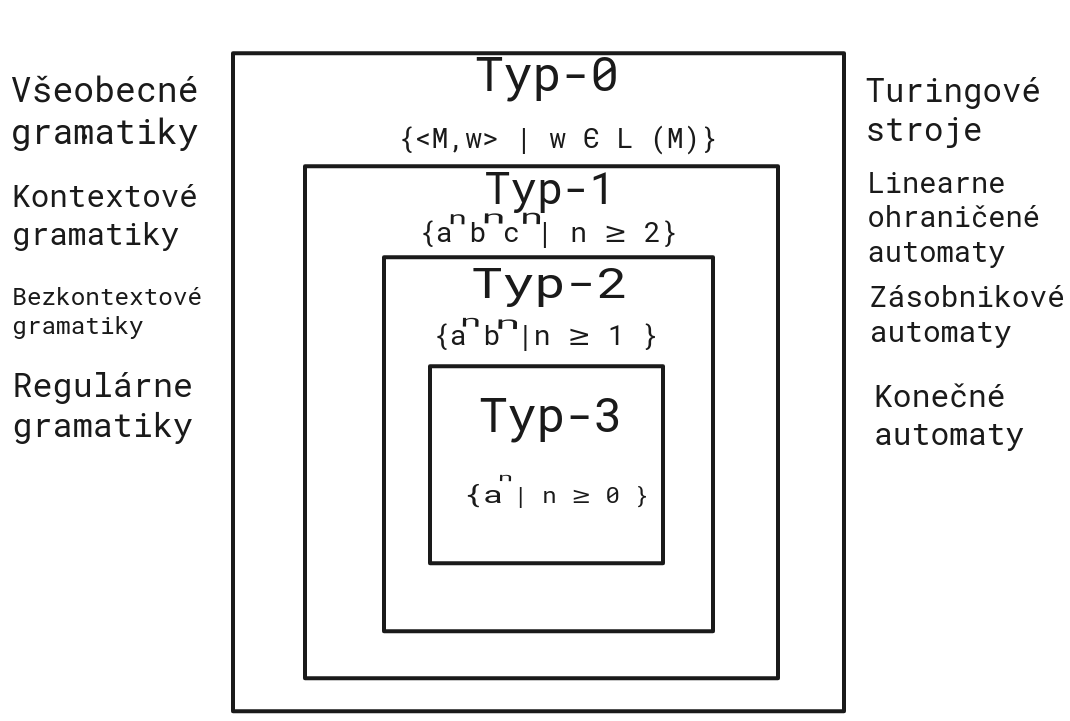
\includegraphics[scale=0.4]{obrazky-figures/ChomHier.png}
    \caption{Chomského hierarchia slabej generativnej kapacity.}
    \label{fig:repetition}
\end{figure}

\subsection*{Typ-3 (Regulárne jazyky)}
Regulárne jazyky sa používajú napríklad pre zápis regulárnych výrazov. Tie sa využívajú v rôznych UNIX-ových nástrojoch. Tieto jazyky sú výpočtovo nenáročné, deterministicky spracovateľné v lineárnom čase a podporujú rôzne matematické operácie, ako sú napríklad zjednotenie alebo konkatenacia. Ich najväčšia nevýhoda oproti silnejším formálnym modelom je ich limitovaná generatívna kapacita.

Regulárne gramatiky sú taktiež veľmi limitujúce v tom, že nedokážu vytvoriť viacúrovňovú stromovú štruktúru, ktorou hudobná štruktúra určite je. Je to kvôli obmedzeniu gramatiky, u ktorej musí byť jeden neterminal na pravej strane produkčných pravidiel. Spracovanie hudobnej štruktúry si vyžaduje minimálne možnosť spracovať vnorené závislosti, ktoré sa v hudbe vyskytujú. Túto možnosť regulárne gramatiky neponúkajú. Príkladom stromovej štruktúry môže byť variácia na obrázku \ref{fig:Preklopenie}.

Markovské procesy, ktoré boli charakterizované Chomskym ako gramatika typu-3 nepreukázali schopnosť spracovať frázovú štruktúru. Tieto limitácie nesúvisia s problematikou stochastických procesov a deterministických procesov. Limitácie sa týkajú produkčných pravidiel. Markovské procesy sa riadia lineárnymi krokovými pravidlami narozdiel od bezkontextových gramatík. Bezkontextové gramatiky umožňujú vytvoriť reťazec neterminálov naraz pomocou produkčných pravidiel. Na základe týchto skutočností vieme, že regulárne gramatiky neponúkajú vhodne riešenie k popisu hudobnej štruktúry.

\subsection*{Typ-2 (Bezkontextové jazyky)}
Tieto jazyky sa vyznačujú štruktúrami, ktoré sú reprezentované balancovanými stromami a ďalšími zrkadliacimi sa štruktúrami. Obrovské využitie týchto jazykov je u programovacích jazykoch, ktoré sú ich deterministický spracovateľnou podmnožinou. Jazyky typu-2 prinášajú so sebou nejednoznačnosť a neplatia u nich operácie doplnok, prienik a ďalšie. Tieto jazyky sú spracovateľné v $O(n^3)$ čase.

Určité časti hudobnej štruktúry, ktoré sú reprezentované hudobným jazykom vieme zaradiť medzi bezkontextové jazyky. Ide o motív alebo tému, ktorá postupne rastie a následne rovnakými tonami klesá. Tento jav tvorí zrkadlovú štruktúru, ktorá je zobrazená na ľavej strane obrázku \ref{fig:dependencies}.

Tieto gramatiky sú jednoduchšie na spracovanie oproti gramatikám, ktoré tvoria jazyky v nadchádzajúcich sekciách. Je to vďaka tomu, že umožňujú reťazce iba na jednej strane produkčných pravidiel. Zložitosť je teda lineárna k počtu neterminálov v derivácií. Sila bezkotextových gramatik leží v tom, že umožňujú reprezentáciu viacúrovňových vnorených syntaktických štruktúr. Neterminal, ktorý môže reprezentovať motív, frázu, vetu alebo sekciu generuje reťazec tokenov na nižšej úrovni. Schopnosť generovať reťazce tokenov v jednom z produkčných pravidiel, ich robí lepším kandidátom k popisu hudobnej štruktúry, narozdiel od regulárnych gramatík.

\begin{figure}[H]
    \centering
    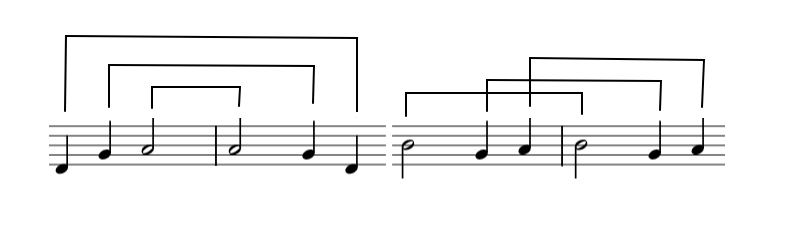
\includegraphics[scale=0.4]{obrazky-figures/zavislosti.png}
    \caption{Znázornenie vnorených a kopírujúcich sa závislosti na variáciach.}
    \label{fig:dependencies}
\end{figure}

\subsection*{Typ-1 (Kontextové jazyky)}
Kontextové jazyky zahrňujú v sebe aj kopírovacie jazyky. Tieto jazyky sú rozhodnutelné, ale vyžadujú si vysokú výpočtovú silu vo väčšine prípadov. Ukázalo sa, že v niektorých prípadoch hudobné jazyky si vyžadujú silnejší formalizmus, ako sú bezkontextové gramatiky. Je to vďaka tomu, že tóny sú medzi jednotlivými taktami sú usporiadané vo forme kopírovacích jazykov. Ukážka takéhoto jazyka v notovom zápise je na pravej strane obrázka \ref{fig:dependencies}.

S kontextovými gramatikami prichádzajú aj problémy. Prvý problém je, že reťazce vygenerovane touto gramatikou sú nerozhodnutelné. Nerozhodné pravidlá sú súčasťou tejto gramatiky, čo znemožňuje zachovanie rovnakej frázovej štruktúry v reťazcoch generovaných kontextovou gramatikou. To je spôsobené tým, že každá strana z produkčných pravidiel môže byť reťazec tokenov. Reťazce tokenov na každej strane znemožňujú aplikáciu kontextových gramatik v analýze hudobnej štruktúry. Bezkontextové gramatiky môžu mať tiež nerozhodné pravidlá, ale krokovanie ich derivácií je zjednodušené. Zjednodušením je hociaký terminál, ktorý sa redukuje na jediný neterminal narozdiel od kontextových gramatik. U kontextových gramatík sa môže redukovať na celý reťazec.

Druhým problémom je implementácia. Použitie prekladača na takúto gramatiku by spôsobuje znásobenie počtu produkčných pravidiel počtom kontextových možnosti. Špecifikácia takejto gramatiky nie je jednoducha. Popisovanie krokov gramatiky takého prekladača sa stane kombinatorické, pretože krížové závislosti musia byť vložené do produkčných tabuliek.

Napriek všetkým týmto komplikáciám je stále možné kontextové závislosti zabudovať do gramatiky konštruovanej čisto z bezkontextových produkčných pravidiel. Tento spôsob je možné celkom jednoznačne preložiť. Problem môže nastať u zobrazovaní kopírovacích závislostiach v gramatike.

\subsection*{Typ-0 (Rekurzívne vyčísliteľné jazyky)}
Rekurzívne vyčísliteľné jazyky sú jazyky, ktoré sú tvorené všeobecnými gramatikami. Tieto gramatiky nezavádzajú žiadne obmedzenia na produkčné pravidla. Z definície tieto gramatiky umožňujú vznik nekonečných reťazcov, ktoré samotné v hudbe nepredstavujú zmysel a nevedú tak k rozumnému riešeniu. Existujú, ale hudobné prostredia, ktoré sa zaoberajú generovaním a syntézou v reálnom čase. Tieto prostredia sú turingovo úplne a volia si silnú generatívnu kapacitu. Problém s výpočtovou náročnosťou nechávajú v rukách užívateľa.

\chapter{Gramatiky s rozptýleným kontextom a ich aplikácia v hudbe}

\chapter{Implementácia}

\chapter{Záver}